
%===========================================================
\section{Experiments}
\label{section:experiments}
In this section, we introduce our detailed implementation and report the performance of our proposed algorithm.

\subsection{Dataset}
  
In our experiments, we use Massachusetts Buildings Dataset (\textit{Mass. Buildings}) proposed by Mnih~\cite{Mnih2013Machine}.
% and publicly available on website \url{http://www.cs.toronto.edu/~vmnih/data/}. 
The dataset consists of 151 aerial images of the Boston area, with each image being 1500$\times$1500 pixels for an area of 2.25 square kilometers. 
The entire dataset covers roughly 340 square kilometers. 
The intensity of each aerial image is scaled into the range of $[0,1]$.
%
The data is split into a training set of 137 images, a test set of 10 images and a validation set of 4 images. 
To train the network, we create a set of image tiles for training and validation by cropping each aerial image using a sliding window with size of 256$\times$256 pixels and stride of 64 pixels.
%
 After scanning, the training and validation datasets include 75938 tiles and 2500 tiles respectively, with their corresponding building masks. 
For testing, we use ten 1500$\times$1500 images excluded from the training images.
%  

\subsection{Training Settings}
 
The implementation of our network is based on the \textit{Caffe}  Library~\cite{Jia2014Caffe}. Our HF-FCN is fine-tuned from an initialization with the pre-trained VGG16 Net model and trained in an end-to-end manner. It is trained using the stochastic gradient descent algorithm, with the hyper-parameters listed in Table~\ref{tab:paramerters}. 
%
The learning rate is divided by 10 for each 8000 iterations.
We find that the learned deconvolutions provide no noticeable improvements in our experiments, similar as \cite{Long2014Fully,Holistically2015}. Therefore, lr$\_$mult is set to zero for all deconvolutional layers.  
%
Except that the pad of first convolutional layer is set to 35, the others are set to 1, same as VGG16 Net. 
%
It takes about six hours to train our network on a single NVIDIA Titan 12GB GPU.
\begin{table}
	\centering
	\caption{Parameters for network training.}
		\begin{tabular}{r|c}
		\hline
		mini-batch size & 18 \\
		initial learning rate & $10^{-5}$\\
		momentum & 0.9\\
		weight decay & 0.02\\
		clip$\_$gradients & 10000 \\
		the number of training iterations & 16000\\		
		\hline
		\end{tabular}
	\label{tab:paramerters} 
\end{table}


\subsection{Results}
 
To show the effectiveness of HF-FCN, we compare our method with two state-of-the-art approaches~\cite{Mnih2013Machine,Saito2016Multiple}.
Three common metrics are used to evaluate the performance of our algorithm: (1) the relaxed precision and recall scores with $\rho = 3$; (2) the standard precision and recall scores ($\rho= 0$); (3) the time cost.  
The relaxed precision is defined as the fraction of detected pixels that are within $\rho$ pixels of a true pixel, while the relaxed recall is defined as the fraction of the true pixels that are within $\rho$ pixels of a detected pixel.
%
The slack parameter $\rho$ is set to 3, which is the same value as used in \cite{Mnih2013Machine,Saito2016Multiple}. 
The relaxed precision-recall curves generated from different methods are shown in Fig.~\ref{fig:relaxedcurve}. As can be seen, all curves of ours are located above others in building prediction obviously.
%
More strictly, we set slack parameter $\rho$ as 0, that is to say, it becomes a standard precision and recall scores. 
%
The precision-recall curves generated from different methods are shown in Fig.~\ref{fig:standardcurve}. We can see that our approach is more appropriate for detecting rooftops in complex scene,  which significantly outperforms  \cite{Mnih2013Machine,Saito2016Multiple}.
%
To compare the system efficiency, we calculate the average time of processing ten test images in the same computer using different methods. 
Table~\ref{tab:PerformanceComparision} shows that our method is able to not only significantly improve the performance, but also dramatically reduces the time cost. 
      
\begin{figure}
\centering
\subfigure[Slack parameter $\rho$ = 3]{	
	\label{fig:relaxedcurve}
	\includegraphics[width=59mm]{figs/PrecisionRecallCurve_3}}
\subfigure[Slack parameter $\rho$ = 0]{
	\label{fig:standardcurve}
	\includegraphics[width=59mm]{figs/PrecisionRecallCurve_0}}
\caption{The relaxed precision-recall curves from different methods with two slack parameters.}
\label{fig:}
\end{figure}
 
    \begin{table} 
    \centering
	\caption{Performance comparison with \cite{Mnih2013Machine,Saito2016Multiple}. Recall here  means recall at breakeven points. Time is computed in the same computer with a single NVIDIA Titan 12GB GPU.}
	\begin{tabular}{L{38mm}C{26mm}C{26mm}C{26mm}}     
	\toprule
	& Recall ($\rho$ = 3) & Recall ($\rho$ = 0)& Time (s)\\
	\midrule
	Mnih-CNN \cite{Mnih2013Machine} & 0.9271 & 0.7661 & 8.70  \\ 
	Mnih-CNN+CRF \cite{Mnih2013Machine} & 0.9282 & 0.7638 & 26.60\\ 
	Saito-multi-MA \cite{Saito2016Multiple} & 0.9503 & 0.7873 & 67.72 \\
	Saito-multi-MA$\&$CIS \cite{Saito2016Multiple} & 0.9509 & 0.7872 & 67.84 \\
	Ours (HF-FCN) & $\bm{0.9643}$ & $\bm{0.8424}$ & $\bm{1.07}$\\
	\bottomrule
	\end{tabular}
	\label{tab:PerformanceComparision}
	\end{table}  
 
 	 
\begin{figure}
\centering
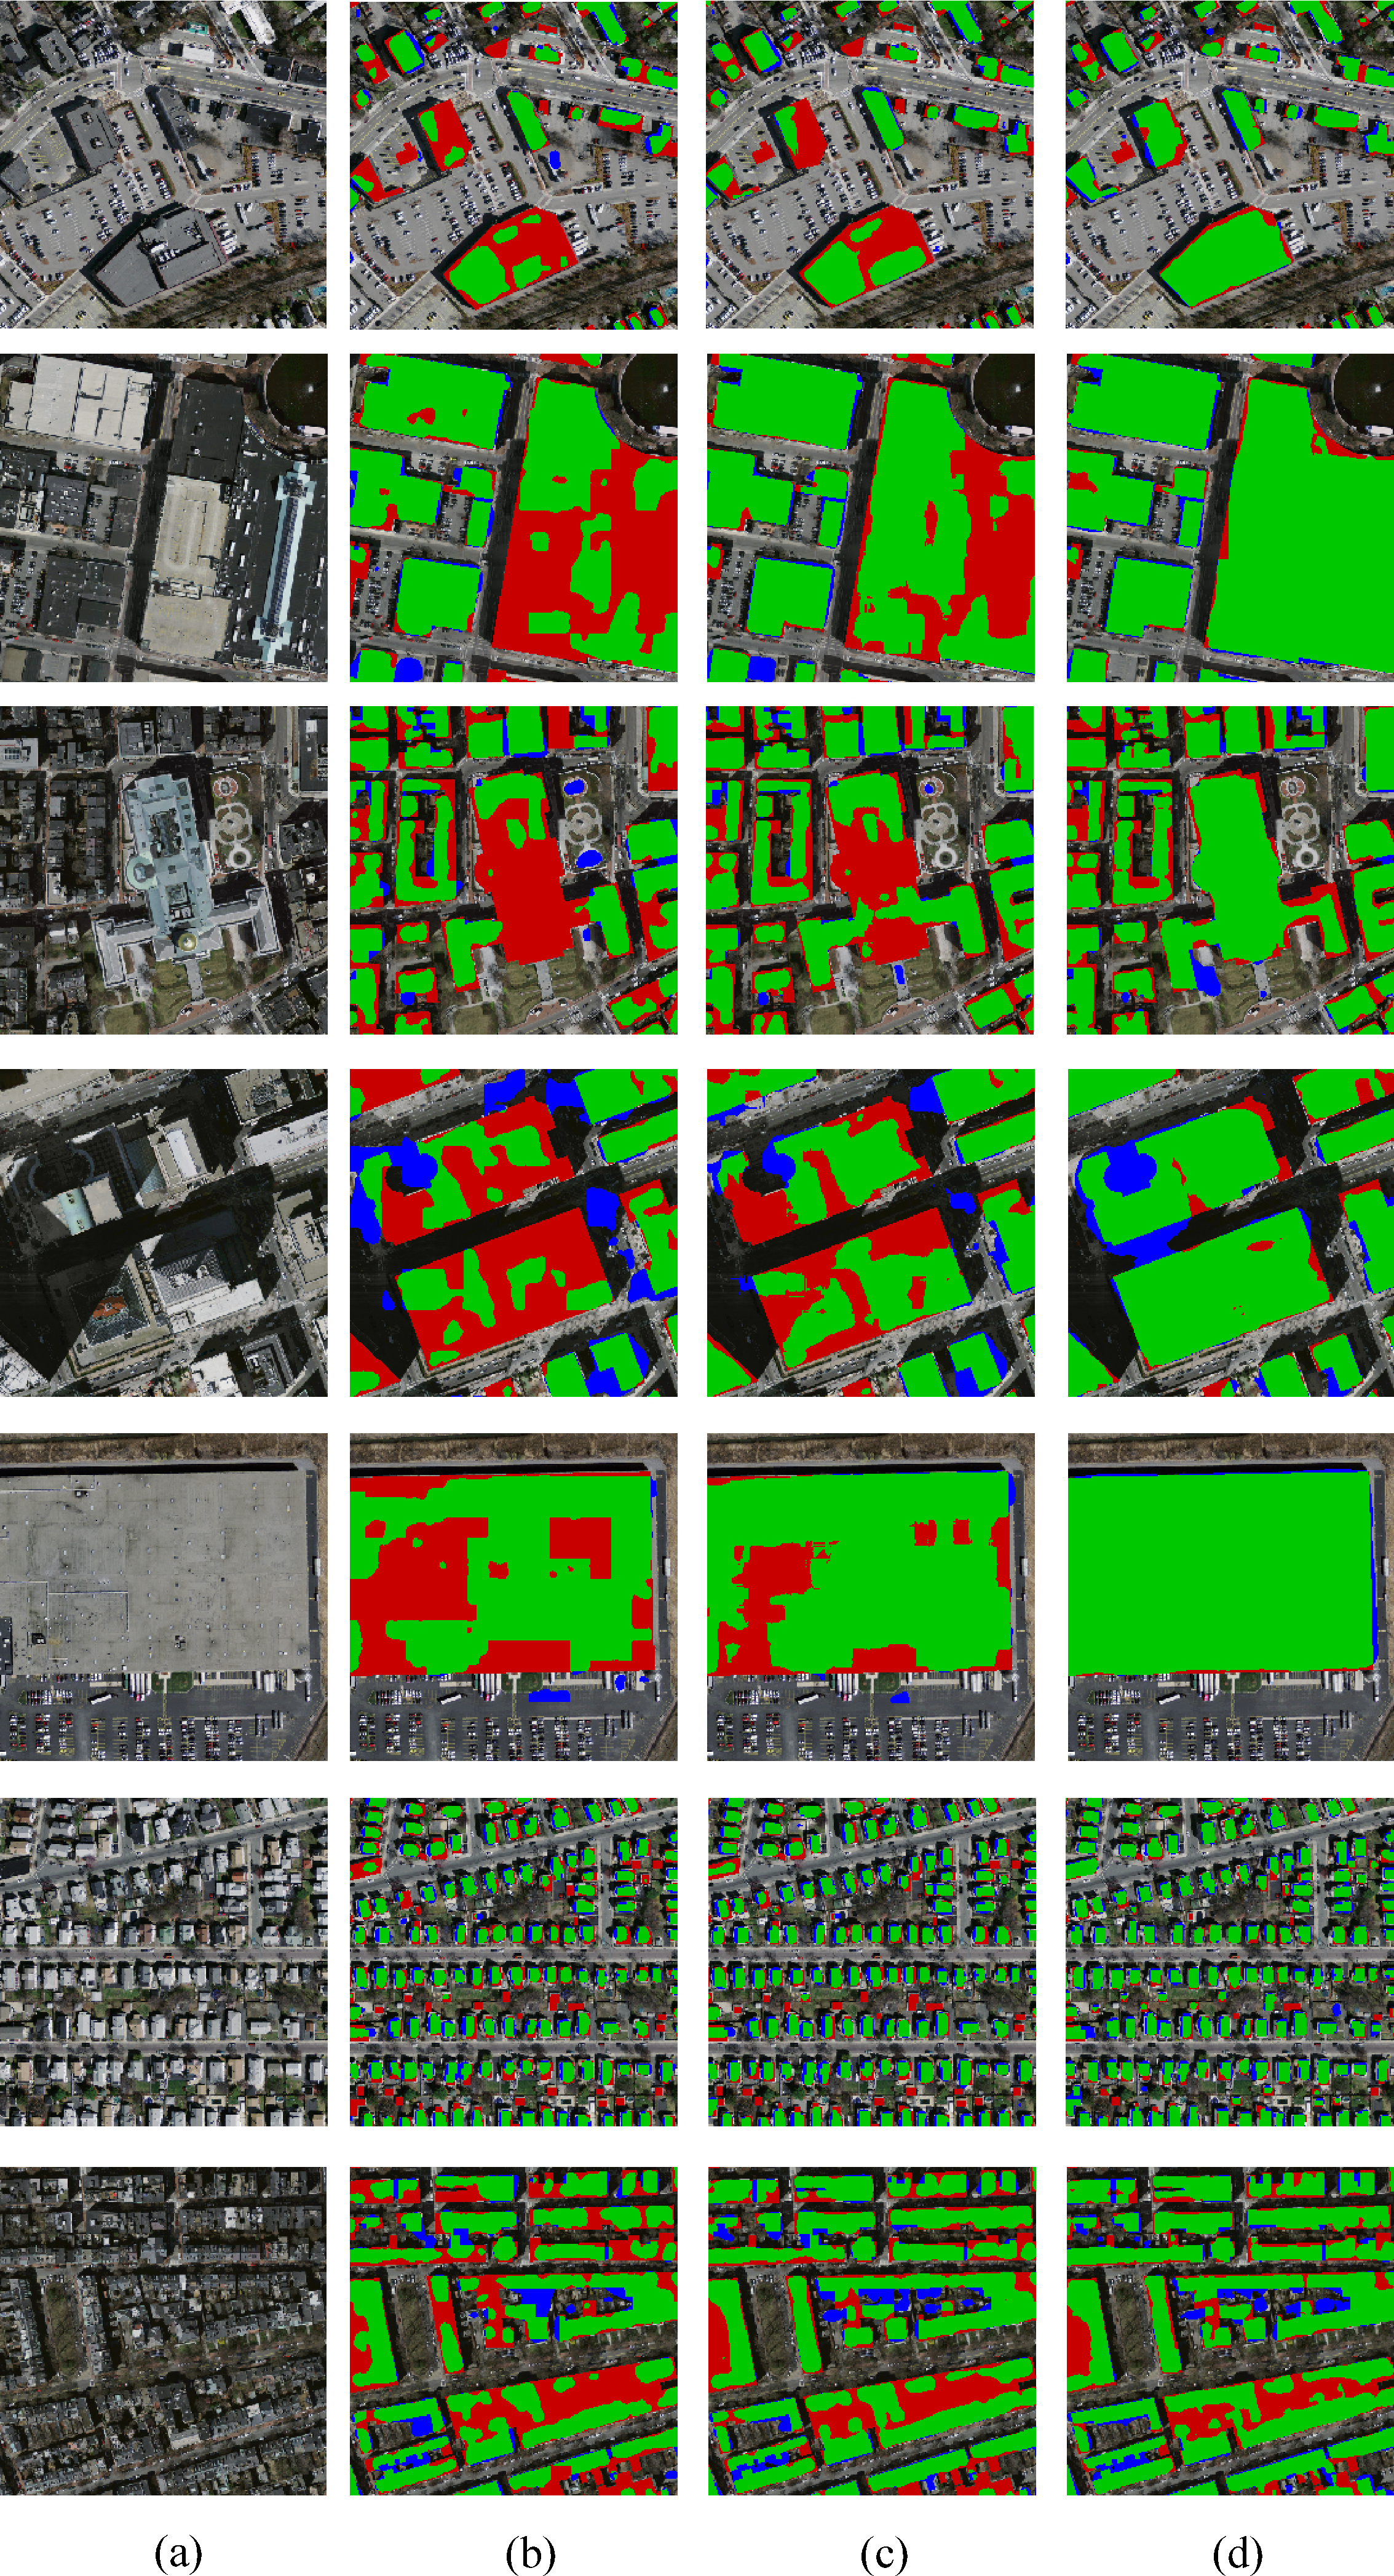
\includegraphics[width=110mm]{figs/ComparedResults}
\caption{(a) Input images. (b) Results of Mnih-CNN+CRF \cite{Mnih2013Machine}. (c) Results of Saito-multi-MA$\&$CIS \cite{Saito2016Multiple}. (d) Our results. 
Correct results (TP) are shown in green, false positives (FP) are shown in blue, and false negatives (FN) are shown in red.}
\label{fig:ComparedResults}
\end{figure} 
    
 
To prove that our network has strong ability in extracting buildings with variant appearances, arbitrary sizes, occlusions, a new experiment is designed.
% 
We crop seven 256$\times$256 image patches that have buildings with variant appearances or occlusions from the test images. 
Corresponding predictions are directly  cropped from the predicted images generated by three approaches, including Mnih-CNN+CRF~\cite{Mnih2013Machine}, Saito-multi-MA$\&$CIS~\cite{Saito2016Multiple} and ours. 
We binarize the probability map using a threshold of 0.5. A series of examples is shown in Fig.~\ref{fig:ComparedResults}.
%
In addition, Table~\ref{tab:ComparedResultsRecall} shows the resulting recalls at the breakeven points of the standard precision recall curve for each patch. The accuracy of our approach is 12.7\% , 6.0\% higher than \cite{Mnih2013Machine},\cite{Saito2016Multiple}, receptively.
 

	\begin{table} 
    \centering
	\caption{Recall at the selected regions of the test images.}
	\begin{tabular}{L{38mm}*{9}{C{9mm}}}     
	\toprule
	Image ID & 01 & 02 & 03 &04 &05 & 06 &07 & mean\\
	\midrule
	Mnih-CNN+CRF~\cite{Mnih2013Machine} & 0.784 & 0.869 & 0.769 & 0.653 & 0.893 & 0.764 & 0.800 & 0.784\\
	Saito-multi-MA$\&$CIS~\cite{Saito2016Multiple} & 0.773 & 0.915 & 0.857 & 0.789 & 0.945 & 0.773 &0.830 & 0.851\\
	Ours (HF-FCN) & $\bm{0.874}$ & $\bm{0.964}$  & $\bm{0.899}$ & $\bm{0.901}$ & $\bm{0.986}$ & $\bm{0.840}$ &  $\bm{0.851}$ & $\bm{0.911}$\\
	\bottomrule
	\end{tabular}
	\label{tab:ComparedResultsRecall}
	\end{table} 
 	 
